% Informe en formato APA 7 (clase apa7, modo manuscrito profesional).
%
% Compilación (desde la carpeta informe/):
%   latexmk -pdf informe_yacimientos_oro.tex
% o bien:
%   pdflatex informe_yacimientos_oro
%   biber    informe_yacimientos_oro
%   pdflatex informe_yacimientos_oro
%   pdflatex informe_yacimientos_oro
%
% Paquetes TeX necesarios: apa7, biblatex-apa (con biber), babel-spanish,
% booktabs, threeparttable, listings.

\documentclass[man,12pt,a4paper,floatsintext,donotrepeattitle]{apa7}

\usepackage[utf8]{inputenc}
\usepackage[T1]{fontenc}
\usepackage{lmodern}
\usepackage[spanish,es-tabla,es-nodecimaldot,es-noshorthands,es-noquoting]{babel}
\usepackage{csquotes}
\usepackage[style=apa,backend=biber]{biblatex}
\addbibresource{referencias.bib}
\setlength{\headheight}{15.4pt}
% Interlineado sencillo dentro de tablas y figuras (permitido por APA 7)
\newcommand{\interlineadosencillo}{\renewcommand{\baselinestretch}{1}\selectfont}

\usepackage{graphicx}
\graphicspath{{../datos/}}
\usepackage{booktabs}
\usepackage{threeparttable}
\usepackage{listings}
\lstset{
  basicstyle=\ttfamily\small,
  columns=fullflexible,
  breaklines=true,
  frame=single,
  framerule=0.4pt,
  xleftmargin=0.5em,
  xrightmargin=0.5em,
  aboveskip=1em,
  belowskip=1em
}

\title{Identificación y distribución territorial de los yacimientos mineros de oro del Perú a partir de GEOCATMIN}
\shorttitle{Yacimientos de oro del Perú}

% Ajuste el autor y la afiliación según corresponda.
\authorsnames{Marcelo Malca}
\authorsaffiliations{{Afiliación institucional}}

\authornote{
  Los datos, el código en Python y R, las tablas y el mapa descritos en este
  informe se encuentran en el repositorio \texttt{marcelomalca/myrep}.
  La correspondencia relacionada con este informe debe dirigirse a Marcelo Malca.
}

\abstract{Este informe describe el proceso seguido para descargar, filtrar,
clasificar y cartografiar los yacimientos mineros de oro del Perú registrados
por el Instituto Geológico, Minero y Metalúrgico (INGEMMET) en su sistema
GEOCATMIN. Se descargaron los 1672 registros de la capa Yacimientos Mineros del
servicio metalogenético mediante su interfaz REST, resolviendo previamente un
error de verificación del certificado SSL del servidor sin desactivar dicha
verificación. A partir del campo de elementos principales se seleccionaron 1030
yacimientos cuyo primer elemento principal es el oro (Au). Estos se agregaron por
departamento, provincia y distrito usando los códigos de ubigeo del Instituto
Nacional de Estadística e Informática (INEI) y se representaron en un mapa
coroplético distrital elaborado en R. Se describe además la procedencia de los
datos: la base es compilada por la Dirección de Recursos Minerales y Energéticos
de INGEMMET a partir de fuentes secundarias, y cada registro representa una mina,
proyecto, prospecto u ocurrencia. Los yacimientos de oro se distribuyen en 22
departamentos, 125 provincias y 358 distritos. Arequipa (15.4\,\%), Madre de Dios
(14.1\,\%), La Libertad (10.2\,\%) y Puno (9.6\,\%) concentran casi la mitad del
total, y la provincia de Tambopata reúne por sí sola 116 yacimientos. Se discuten
las limitaciones del procedimiento, entre ellas el desfase entre los límites
distritales disponibles y la división política vigente.}

\keywords{GEOCATMIN, INGEMMET, yacimientos de oro, Perú, cartografía coroplética, R}

\begin{document}
% Etiquetas en español según APA 7 (la configuración de apa7 usa mayúsculas)
\renewcommand{\keywordname}{Palabras clave}
\renewcommand{\acksname}{Nota del autor}
\hypersetup{hidelinks}
\maketitle

\section*{Identificación y distribución territorial de los yacimientos mineros de oro del Perú a partir de GEOCATMIN}

El Perú es uno de los principales productores de oro de América Latina, y la
información sobre la ubicación de sus yacimientos es un insumo básico para la
planificación territorial, la exploración minera y la investigación geológica.
El Instituto Geológico, Minero y Metalúrgico (INGEMMET) publica esta información
en GEOCATMIN, su sistema de información geológica y catastral, que puede
consultarse en un visor web o mediante servicios de mapas ArcGIS.

El objetivo de este trabajo fue obtener, de forma reproducible, el inventario de
yacimientos mineros del Perú registrados en GEOCATMIN; identificar aquellos cuyo
elemento principal es el oro; cuantificarlos por departamento, provincia y
distrito; y representar su distribución en un mapa a nivel distrital. El informe
describe cada etapa del proceso, las decisiones metodológicas adoptadas y las
limitaciones de los resultados.

\section{Método}

\subsection{Fuente de datos}

Los yacimientos se obtuvieron de la capa \textit{Yacimientos Mineros} (capa 1)
del servicio de mapas \texttt{SERV\_METALOGENETICO} de GEOCATMIN
\parencite{ingemmet2026}, publicado en ArcGIS Server versión 10.91. La capa
contiene geometrías de tipo punto y 78 campos de atributos, entre ellos el
nombre de la unidad minera (\texttt{UNIDAD}), el tipo de yacimiento
(\texttt{T\_YACIM}), las coordenadas geográficas (\texttt{LATITUD},
\texttt{LONGITUD}), los códigos de ubicación política (\texttt{REGION},
\texttt{PROVINCIA}, \texttt{DISTRITO}) y los elementos principales y
acompañantes (\texttt{ELE\_PRINC}, \texttt{ELE\_ACOMPA}). La consulta se realizó
el 12 de octubre de 2026.

Como fuentes complementarias se emplearon (a) los límites distritales del Perú
en formato GeoJSON, derivados de la cartografía del INEI, con 1834 polígonos
\parencite{juaneladio-geojson}, y (b) la tabla de códigos de ubigeo del INEI con
los nombres de departamentos, provincias y distritos, que incluye 1895 distritos
\parencite{castagnetto-ubigeo}.

\subsection{Procedencia de los datos}

Esta sección describe cómo se generan los datos de la capa de yacimientos, según
la documentación publicada por INGEMMET y el contenido de los propios registros.
Comprender su origen es necesario para interpretar correctamente qué representa
cada punto y qué no.

\subsubsection{Institución responsable}

La información es producida por INGEMMET, organismo técnico adscrito al sector
Energía y Minas. Dentro de la institución, la base de datos de yacimientos fue
desarrollada por el Programa de Metalogenia de la Dirección de Recursos
Minerales y Energéticos (DRME) \parencite{huanacuni2010guia}. Esta base es el
insumo del Mapa Metalogenético del Perú, cuya versión 2020 fue elaborada por el
mismo equipo \parencite{acosta2020}. Su gestión informática se
desarrolló junto con la Oficina de Sistemas de Información de INGEMMET a partir
de 2007, en el denominado Módulo del Mapa Metalogenético
\parencite{huanacuni2010cpg}. Los registros conservan el código del proyecto que
los originó (\texttt{CD\_PROY}), que es el mismo para toda la capa, y los campos
\texttt{RESPONS} y \texttt{REVISADO} identifican al profesional responsable y,
cuando existe, al revisor de cada registro.

\subsubsection{Forma de recolección}

La base no proviene de un censo ni de una encuesta, sino de la
\textit{compilación, actualización y validación} de información de fuentes
secundarias \parencite{huanacuni2010cpg}. Según INGEMMET, las fuentes son los
anuarios y reportes anuales del Ministerio de Energía y Minas, las memorias de
compañías mineras, los boletines e informes técnicos del propio INGEMMET, los
estudios de franjas metalogenéticas, los artículos de revistas especializadas en
geología económica, las tesis universitarias y la prensa especializada del sector
minero \parencite{huanacuni2010guia,ingemmet2026servicio}. En algunos
yacimientos, la información se complementa con estudios de laboratorio de
muestras de la litoteca institucional (descripciones petrográficas,
mineragráficas y espectrales), aunque esto ocurre solo en ocho registros de toda
la capa.

INGEMMET clasifica la confiabilidad de la información según su fuente en tres
niveles: (1) reportes oficiales, boletines, memorias de empresas, artículos
científicos y tesis; (2) notas de la prensa especializada; y (3) comunicaciones
verbales de profesionales del sector. Según INGEMMET, más del 90\,\% de los
datos están validados y son de alta calidad, y el resto son datos referenciales
de notas de prensa y comunicaciones verbales \parencite{ingemmet2026servicio}. En 2010 se indicaba que la base se
actualizaba semestralmente \parencite{huanacuni2010cpg}. Además, INGEMMET invita a
los usuarios a enviar observaciones y correcciones por correo electrónico
\parencite{huanacuni2010guia}.

\subsubsection{Unidad de observación}

Cada registro de la capa es un \textit{punto} que representa la ubicación de una
concentración mineral conocida: una mina, un proyecto, un prospecto o una
ocurrencia. En algunos casos, el punto representa un distrito minero que agrupa
varias unidades, como Orcopampa o Yanacocha \parencite{ingemmet2026servicio}. El
término \textit{yacimiento}, tal como se usa en la capa y en este informe,
abarca por lo tanto situaciones económicas muy distintas, que la base distingue
en el campo \texttt{COD\_TIPO}. La Tabla~\ref{tab:tipos} resume la composición de
los 1030 registros de oro analizados y las definiciones de INGEMMET.

\begin{table}[htbp]
\caption{Yacimientos de oro según tipo de registro}
\label{tab:tipos}
\centering
\interlineadosencillo
\begin{threeparttable}
\small
\begin{tabular}{@{}lrrp{8.2cm}@{}}
\toprule
Tipo & $n$ & \% & Definición de INGEMMET \\
\midrule
Ocurrencia & 361 & 35.0 & Concentración natural de minerales de interés
económico cuya explotación no sería rentable bajo las condiciones
prevalecientes. \\
Mina & 315 & 30.6 & Mina activa donde se extrae mineral, o mina cerrada. \\
Prospecto & 215 & 20.9 & Zona prospectada con resultados de interés
económico que requieren estudios de mayor detalle para confirmarlo. \\
Proyecto & 138 & 13.4 & Depósito en estado avanzado de exploración, con
recursos reconocidos. \\
Yacimiento & 1 & 0.1 & Sin definición publicada. \\
\midrule
Total & 1030 & 100.0 & \\
\bottomrule
\end{tabular}
\vspace{6pt}
\begin{tablenotes}[flushleft]
\small
\item \textit{Nota.} Tipo según el campo \texttt{COD\_TIPO}. Las definiciones
se adaptaron de \textcite{huanacuni2010guia}. Elaboración propia a partir de datos
de GEOCATMIN \parencite{ingemmet2026}.
\end{tablenotes}
\end{threeparttable}
\end{table}

El tipo de depósito (\texttt{T\_YACIM}) sigue una clasificación de INGEMMET en
11 tipos y 50 subtipos, adaptada de Niggli, Lindgren y Schneiderhöhn
\parencite{huanacuni2010guia}. Entre los yacimientos de oro predominan los
depósitos hidrotermales sin clasificación genética (tipo X; 435 registros, de
los cuales 400 son vetas), los depósitos hidrotermales (tipo III; 314 registros,
principalmente epitermales, orogénicos y relacionados con intrusivos) y los
depósitos exóticos (tipo IX; 254 registros, de los cuales 241 son placeres); 23
registros no tienen tipo asignado. Por último, el campo \texttt{ELE\_PRINC} lista
los elementos económicos principales ``ordenados según su importancia''
\parencite{ingemmet2026servicio}, lo que respalda el criterio de selección
descrito más adelante.

\subsubsection{Cobertura temporal}

La capa no es una serie de tiempo ni corresponde a un año de referencia único.
Es un inventario acumulado que se actualiza de forma continua, y cada consulta
devuelve su estado en ese momento. Su antecedente directo es la base de
operaciones y proyectos de oro de 2010, que reunía 1136 registros compilados
hasta abril de ese año \parencite{huanacuni2010guia}. En la capa actual, la
fecha de creación de los registros de oro (\texttt{CREATIONDATE}) va de
noviembre de 2011 a agosto de 2026. El 74.8\,\% se creó en 2012 y el 15.5\,\%
en 2021, lo que sugiere cargas masivas en esos años. Esta fecha corresponde a la
incorporación del registro a la base actual, no necesariamente a la fecha de
la información que contiene. La última edición (\texttt{EDITDATE}) es posterior
a 2020 en 233 registros (22.6\,\%), y 218 registros (21.2\,\%) tienen una fecha
de revisión (\texttt{FECHA\_REV}) entre 2021 y 2026. Los demás no han sido
editados desde 2012--2016. En consecuencia, atributos que cambian en el tiempo,
como el estado de la operación (\texttt{ESTADO}), reflejan la situación a la
fecha de la última actualización de cada registro. La consulta para este
informe se realizó el 12 de octubre de 2026.

\subsubsection{Referencia espacial}

La cobertura es nacional. Según la documentación, las ubicaciones se registran
en coordenadas UTM con datum WGS84, en las zonas 17, 18 y 19
\parencite{ingemmet2026servicio}; de los registros de oro, 571 están en la zona
18, 324 en la 19 y 135 en la 17. El servicio entrega además las coordenadas en
grados decimales (WGS84), que son las que se usaron en este trabajo. La altitud
solo está registrada en 178 casos (17.3\,\%).

\subsubsection{Calidad y completitud de los registros}

La calidad de cada registro está codificada en el campo \texttt{CD\_CALIDAD}. La
capa actual usa cuatro códigos (Calidad-A a Calidad-D), distintos de los tres
niveles numéricos descritos en la documentación, y su equivalencia no está
publicada. Entre los registros de oro, el 95.5\,\% tiene el código Calidad-B, 41
tienen Calidad-C, 3 Calidad-D y 2 Calidad-A. Todos los registros están marcados
como publicables (\texttt{REGISTRO}).

Los campos de identificación, tipo, elementos y ubicación están casi completos,
pero los campos descriptivos tienen una cobertura baja. Entre los registros de
oro, el estado de la operación falta en el 57.2\,\% y la escala de producción
minera (\texttt{CATEGORIA}) en el 75.0\,\%. Solo 47 registros tienen datos de
recursos, 48 de reservas y 30 de producción. Por ello, este informe se limita a
contar registros y no intenta estimar el tamaño ni la importancia económica de
los yacimientos.

\subsection{Herramientas}

La descarga y el filtrado se realizaron en Python~3.13 con las bibliotecas
Requests \parencite{requests}, pandas \parencite{mckinney2010} y GeoPandas
\parencite{geopandas}. La agregación territorial y la cartografía se realizaron
en R \parencite{rcore2024} con los paquetes sf \parencite{pebesma2018}, dplyr
\parencite{dplyr}, readr \parencite{readr} y ggplot2 \parencite{wickham2016}.

\subsection{Procedimiento}

\subsubsection{Identificación del servicio y de la capa}

Se partió de un script en Python preexistente que suponía que los yacimientos
estaban en la capa 3 del servicio metalogenético o en un servicio denominado
\texttt{Temp/SERV\_YACIMIENTO\_MINERO}. Al consultar el catálogo de servicios se
comprobó que este último ya no existe (el servidor responde con el código 404) y
que la capa 3 corresponde a \textit{Área en Operación Minera}. La capa de
yacimientos es la capa 1 del servicio \texttt{SERV\_METALOGENETICO}, por lo que
el script se corrigió en consecuencia.

\subsubsection{Corrección del error de certificado SSL}

Las primeras conexiones al servidor fallaron con el error
\textit{unable to get local issuer certificate}. El análisis de la conexión
mostró que el servidor envía únicamente su propio certificado
(\texttt{*.ingemmet.gob.pe}) y omite el certificado intermedio de la autoridad
emisora (\textit{Sectigo Public Server Authentication CA OV R36}). Los
navegadores web suelen completar esta cadena de forma automática, pero bibliotecas
como Requests no lo hacen. En lugar de desactivar la verificación SSL, lo que
expondría la conexión a ataques de intermediario, se descargó el certificado
intermedio desde la dirección publicada por el propio certificado del servidor y
se incorporó al script. Este se añade al conjunto de autoridades de confianza del
sistema en cada ejecución. El certificado intermedio es válido hasta marzo de
2036.

\subsubsection{Descarga de los registros}

La descarga se realizó en dos pasos mediante la operación \textit{query} de la
interfaz REST de ArcGIS \parencite{esri-query}. Primero se solicitaron
únicamente los identificadores de todos los registros
(\texttt{returnIdsOnly=true}), lo que evita el límite de 2000 registros por
consulta que impone el servicio. Luego se descargaron los atributos y las
geometrías en lotes de 500 identificadores, en formato GeoJSON y en el sistema
de referencia WGS84 (EPSG:4326). Se obtuvieron los 1672 registros de la capa,
que se guardaron en formato CSV y GeoPackage. El número de registros coincidió
con el conteo informado por el servidor.

\subsubsection{Filtrado de los yacimientos de oro}

El campo \texttt{ELE\_PRINC} contiene los elementos principales de cada
yacimiento como una lista de símbolos químicos separados por comas (por ejemplo,
\texttt{Au}, \texttt{Cu,Au} o \texttt{Ag,Pb,Zn}); 18 registros no tienen valor
en este campo. Para evitar falsas coincidencias, la lista se separó en sus
elementos en lugar de buscar el texto \texttt{Au} dentro de la cadena. Se
definieron dos criterios:

\begin{enumerate}
  \item \textit{Oro entre los elementos principales}: el símbolo \texttt{Au}
  aparece en cualquier posición de la lista. Cumplen este criterio 1184
  yacimientos, cifra que coincide con la consulta equivalente ejecutada en el
  servidor (\texttt{ELE\_PRINC LIKE '\%Au\%'}).
  \item \textit{Oro como elemento principal}: \texttt{Au} es el primer elemento
  de la lista. Cumplen este criterio 1030 yacimientos.
\end{enumerate}

Se adoptó el segundo criterio para el análisis, pues el orden de la lista sugiere
la importancia relativa de cada elemento y el criterio responde mejor a la
pregunta de interés. De los 1030 yacimientos seleccionados, 908 tienen el oro como
único elemento principal y los demás lo combinan con plata (52), cobre (45) u
otros elementos.

\subsubsection{Clasificación por departamento, provincia y distrito}

Cada yacimiento se asignó a la unidad territorial indicada por sus códigos de
ubicación en GEOCATMIN (\texttt{REGION}, \texttt{PROVINCIA} y
\texttt{DISTRITO}). Estos códigos siguen el sistema de ubigeo del INEI, de dos,
cuatro y seis dígitos. Los nombres de cada unidad se incorporaron cruzando los
códigos con la tabla de ubigeo, y todos los códigos encontraron correspondencia.
Luego se contó el número de yacimientos por departamento, provincia y distrito, y
los resultados se exportaron en tres tablas en formato CSV.

\subsubsection{Elaboración del mapa}

Los conteos distritales se unieron a los polígonos de límites mediante el código
de ubigeo. Tres yacimientos se encuentran en distritos creados después de la
elaboración de la capa de límites: Kumpirushiato (Cusco), Castillo Grande
(Huánuco) y Santa Lucía (San Martín). Para el mapa, estos tres yacimientos se
asignaron al polígono que contiene su punto, que corresponde al distrito del que
se separaron. En las tablas conservan su código y nombre vigentes.

Dado que la distribución de yacimientos por distrito es muy asimétrica (la mitad
de los distritos tiene un solo yacimiento y el máximo es de 42), se optó por una
escala de colores por clases en lugar de una continua. Con una escala continua,
casi todos los distritos se verían del mismo tono. Se definieron cinco clases (1,
2, 3--4, 5--9 y 10 o más yacimientos) con una paleta secuencial de un solo tono,
de azul claro a azul oscuro. Antes de usarla se verificó con una herramienta de
validación que los tonos fueran monótonos en luminosidad y distinguibles entre
clases contiguas, y que el tono más claro tuviera un contraste suficiente con el
fondo. Los distritos sin yacimientos se representaron en gris neutro y se
superpusieron los límites departamentales como referencia. El mapa se exportó en
formato PNG a 300 ppp.

\section{Resultados}

Los 1030 yacimientos con oro como elemento principal se distribuyen en 22
departamentos, 125 provincias y 358 distritos; no se registran yacimientos de oro
en Tumbes, Ucayali ni en la Provincia Constitucional del Callao. La
Tabla~\ref{tab:departamentos} muestra su distribución por departamento. Arequipa,
Madre de Dios, La Libertad y Puno concentran el 49.3\,\% del total, mientras que
Lambayeque, Loreto y San Martín registran tres yacimientos cada uno.

\begin{table}[htbp]
\caption{Yacimientos mineros de oro por departamento}
\label{tab:departamentos}
\centering
\interlineadosencillo
\begin{threeparttable}
\begin{tabular}{@{}llrr@{}}
\toprule
Código & Departamento & Yacimientos & \% \\
\midrule
04 & AREQUIPA       & 159 & 15.4 \\
17 & MADRE DE DIOS  & 145 & 14.1 \\
13 & LA LIBERTAD    & 105 & 10.2 \\
21 & PUNO           &  99 &  9.6 \\
05 & AYACUCHO       &  81 &  7.9 \\
08 & CUSCO          &  74 &  7.2 \\
03 & APURIMAC       &  56 &  5.4 \\
11 & ICA            &  51 &  5.0 \\
02 & ANCASH         &  47 &  4.6 \\
06 & CAJAMARCA      &  44 &  4.3 \\
10 & HUANUCO        &  29 &  2.8 \\
15 & LIMA           &  28 &  2.7 \\
09 & HUANCAVELICA   &  23 &  2.2 \\
12 & JUNIN          &  21 &  2.0 \\
20 & PIURA          &  21 &  2.0 \\
01 & AMAZONAS       &  12 &  1.2 \\
19 & PASCO          &  12 &  1.2 \\
23 & TACNA          &   9 &  0.9 \\
18 & MOQUEGUA       &   5 &  0.5 \\
14 & LAMBAYEQUE     &   3 &  0.3 \\
16 & LORETO         &   3 &  0.3 \\
22 & SAN MARTIN     &   3 &  0.3 \\
\midrule
   & Total          & 1030 & 100.0 \\
\bottomrule
\end{tabular}
\vspace{6pt}
\begin{tablenotes}[flushleft]
\small
\item \textit{Nota.} Se consideran los yacimientos cuyo primer elemento
principal es el oro (Au). Los nombres se reproducen tal como figuran en la
tabla de ubigeo del INEI. Los porcentajes están redondeados a un decimal.
Elaboración propia a partir de datos de GEOCATMIN \parencite{ingemmet2026}.
\end{tablenotes}
\end{threeparttable}
\end{table}

A nivel provincial (Tabla~\ref{tab:provincias}), Tambopata, en Madre de Dios,
destaca con 116 yacimientos, casi el doble que la segunda provincia, Lucanas
(Ayacucho), con 60. Les siguen Caravelí (Arequipa), Pataz (La Libertad) y
Carabaya (Puno), cada una con entre 48 y 52 yacimientos.

\begin{table}[htbp]
\caption{Las 15 provincias con más yacimientos mineros de oro}
\label{tab:provincias}
\centering
\interlineadosencillo
\begin{threeparttable}
\begin{tabular}{@{}lllr@{}}
\toprule
Código & Provincia & Departamento & Yacimientos \\
\midrule
1701 & TAMBOPATA         & MADRE DE DIOS & 116 \\
0506 & LUCANAS           & AYACUCHO      &  60 \\
0403 & CARAVELI          & AREQUIPA      &  52 \\
1308 & PATAZ             & LA LIBERTAD   &  49 \\
2103 & CARABAYA          & PUNO          &  48 \\
0406 & CONDESUYOS        & AREQUIPA      &  39 \\
2112 & SANDIA            & PUNO          &  34 \\
1103 & NAZCA             & ICA           &  30 \\
0404 & CASTILLA          & AREQUIPA      &  29 \\
1702 & MANU              & MADRE DE DIOS &  29 \\
0812 & QUISPICANCHI      & CUSCO         &  26 \\
1310 & SANTIAGO DE CHUCO & LA LIBERTAD   &  24 \\
2002 & AYABACA           & PIURA         &  18 \\
0307 & GRAU              & APURIMAC      &  17 \\
0408 & LA UNION          & AREQUIPA      &  17 \\
\bottomrule
\end{tabular}
\vspace{6pt}
\begin{tablenotes}[flushleft]
\small
\item \textit{Nota.} La tabla completa, con las 125 provincias, se encuentra en
el archivo \texttt{datos/oro\_por\_provincia.csv}.
Elaboración propia a partir de datos de GEOCATMIN \parencite{ingemmet2026}.
\end{tablenotes}
\end{threeparttable}
\end{table}

A nivel distrital, la distribución está muy concentrada: 185 distritos (51.7\,\%)
registran un solo yacimiento, 68 registran dos, 56 entre tres y cuatro, 31 entre
cinco y nueve, y 18 registran diez o más. Los diez distritos con más yacimientos
reúnen 223 yacimientos, el 21.7\,\% del total. La Tabla~\ref{tab:distritos} lista
los 15 distritos con más yacimientos; los tres primeros (Laberinto, Inambari y
Tambopata) pertenecen a la provincia de Tambopata.

\begin{table}[htbp]
\caption{Los 15 distritos con más yacimientos mineros de oro}
\label{tab:distritos}
\centering
\interlineadosencillo
\begin{threeparttable}
\small
\begin{tabular}{@{}llllr@{}}
\toprule
Ubigeo & Distrito & Provincia & Departamento & Yacimientos \\
\midrule
170104 & LABERINTO     & TAMBOPATA         & MADRE DE DIOS & 42 \\
170102 & INAMBARI      & TAMBOPATA         & MADRE DE DIOS & 41 \\
170101 & TAMBOPATA     & TAMBOPATA         & MADRE DE DIOS & 27 \\
211209 & ALTO INAMBARI & SANDIA            & PUNO          & 21 \\
130809 & PATAZ         & PATAZ             & LA LIBERTAD   & 19 \\
170203 & MADRE DE DIOS & MANU              & MADRE DE DIOS & 17 \\
040606 & RIO GRANDE    & CONDESUYOS        & AREQUIPA      & 14 \\
110303 & EL INGENIO    & NAZCA             & ICA           & 14 \\
130808 & PARCOY        & PATAZ             & LA LIBERTAD   & 14 \\
200210 & SUYO          & AYABACA           & PIURA         & 14 \\
210304 & COASA         & CARABAYA          & PUNO          & 13 \\
081203 & CAMANTI       & QUISPICANCHI      & CUSCO         & 12 \\
210303 & AYAPATA       & CARABAYA          & PUNO          & 12 \\
050621 & SANTA LUCIA   & LUCANAS           & AYACUCHO      & 11 \\
131006 & QUIRUVILCA    & SANTIAGO DE CHUCO & LA LIBERTAD   & 11 \\
\bottomrule
\end{tabular}
\vspace{6pt}
\begin{tablenotes}[flushleft]
\small
\item \textit{Nota.} La tabla completa, con los 358 distritos, se encuentra en
el archivo \texttt{datos/oro\_por\_distrito.csv}.
Elaboración propia a partir de datos de GEOCATMIN \parencite{ingemmet2026}.
\end{tablenotes}
\end{threeparttable}
\end{table}

La Figura~\ref{fig:mapa} muestra la distribución espacial de los yacimientos por
distrito. Se distinguen tres zonas de concentración: (a) la llanura amazónica de
Madre de Dios y su borde con Puno y Cusco, donde se ubican los distritos con más
yacimientos del país; (b) el sur andino y costero, desde Ica y Ayacucho hasta
Arequipa, Apurímac y Puno, con muchos distritos en las clases intermedias; y
(c) el norte andino, en particular la provincia de Pataz y los distritos
vecinos de La Libertad, además de Cajamarca y la sierra de Piura. La Amazonía
norte y central (Loreto, Ucayali y San Martín) casi no registra yacimientos de
oro.

\begin{figure}[htbp]
\caption{Yacimientos mineros de oro por distrito}
\label{fig:mapa}
\centering
\interlineadosencillo
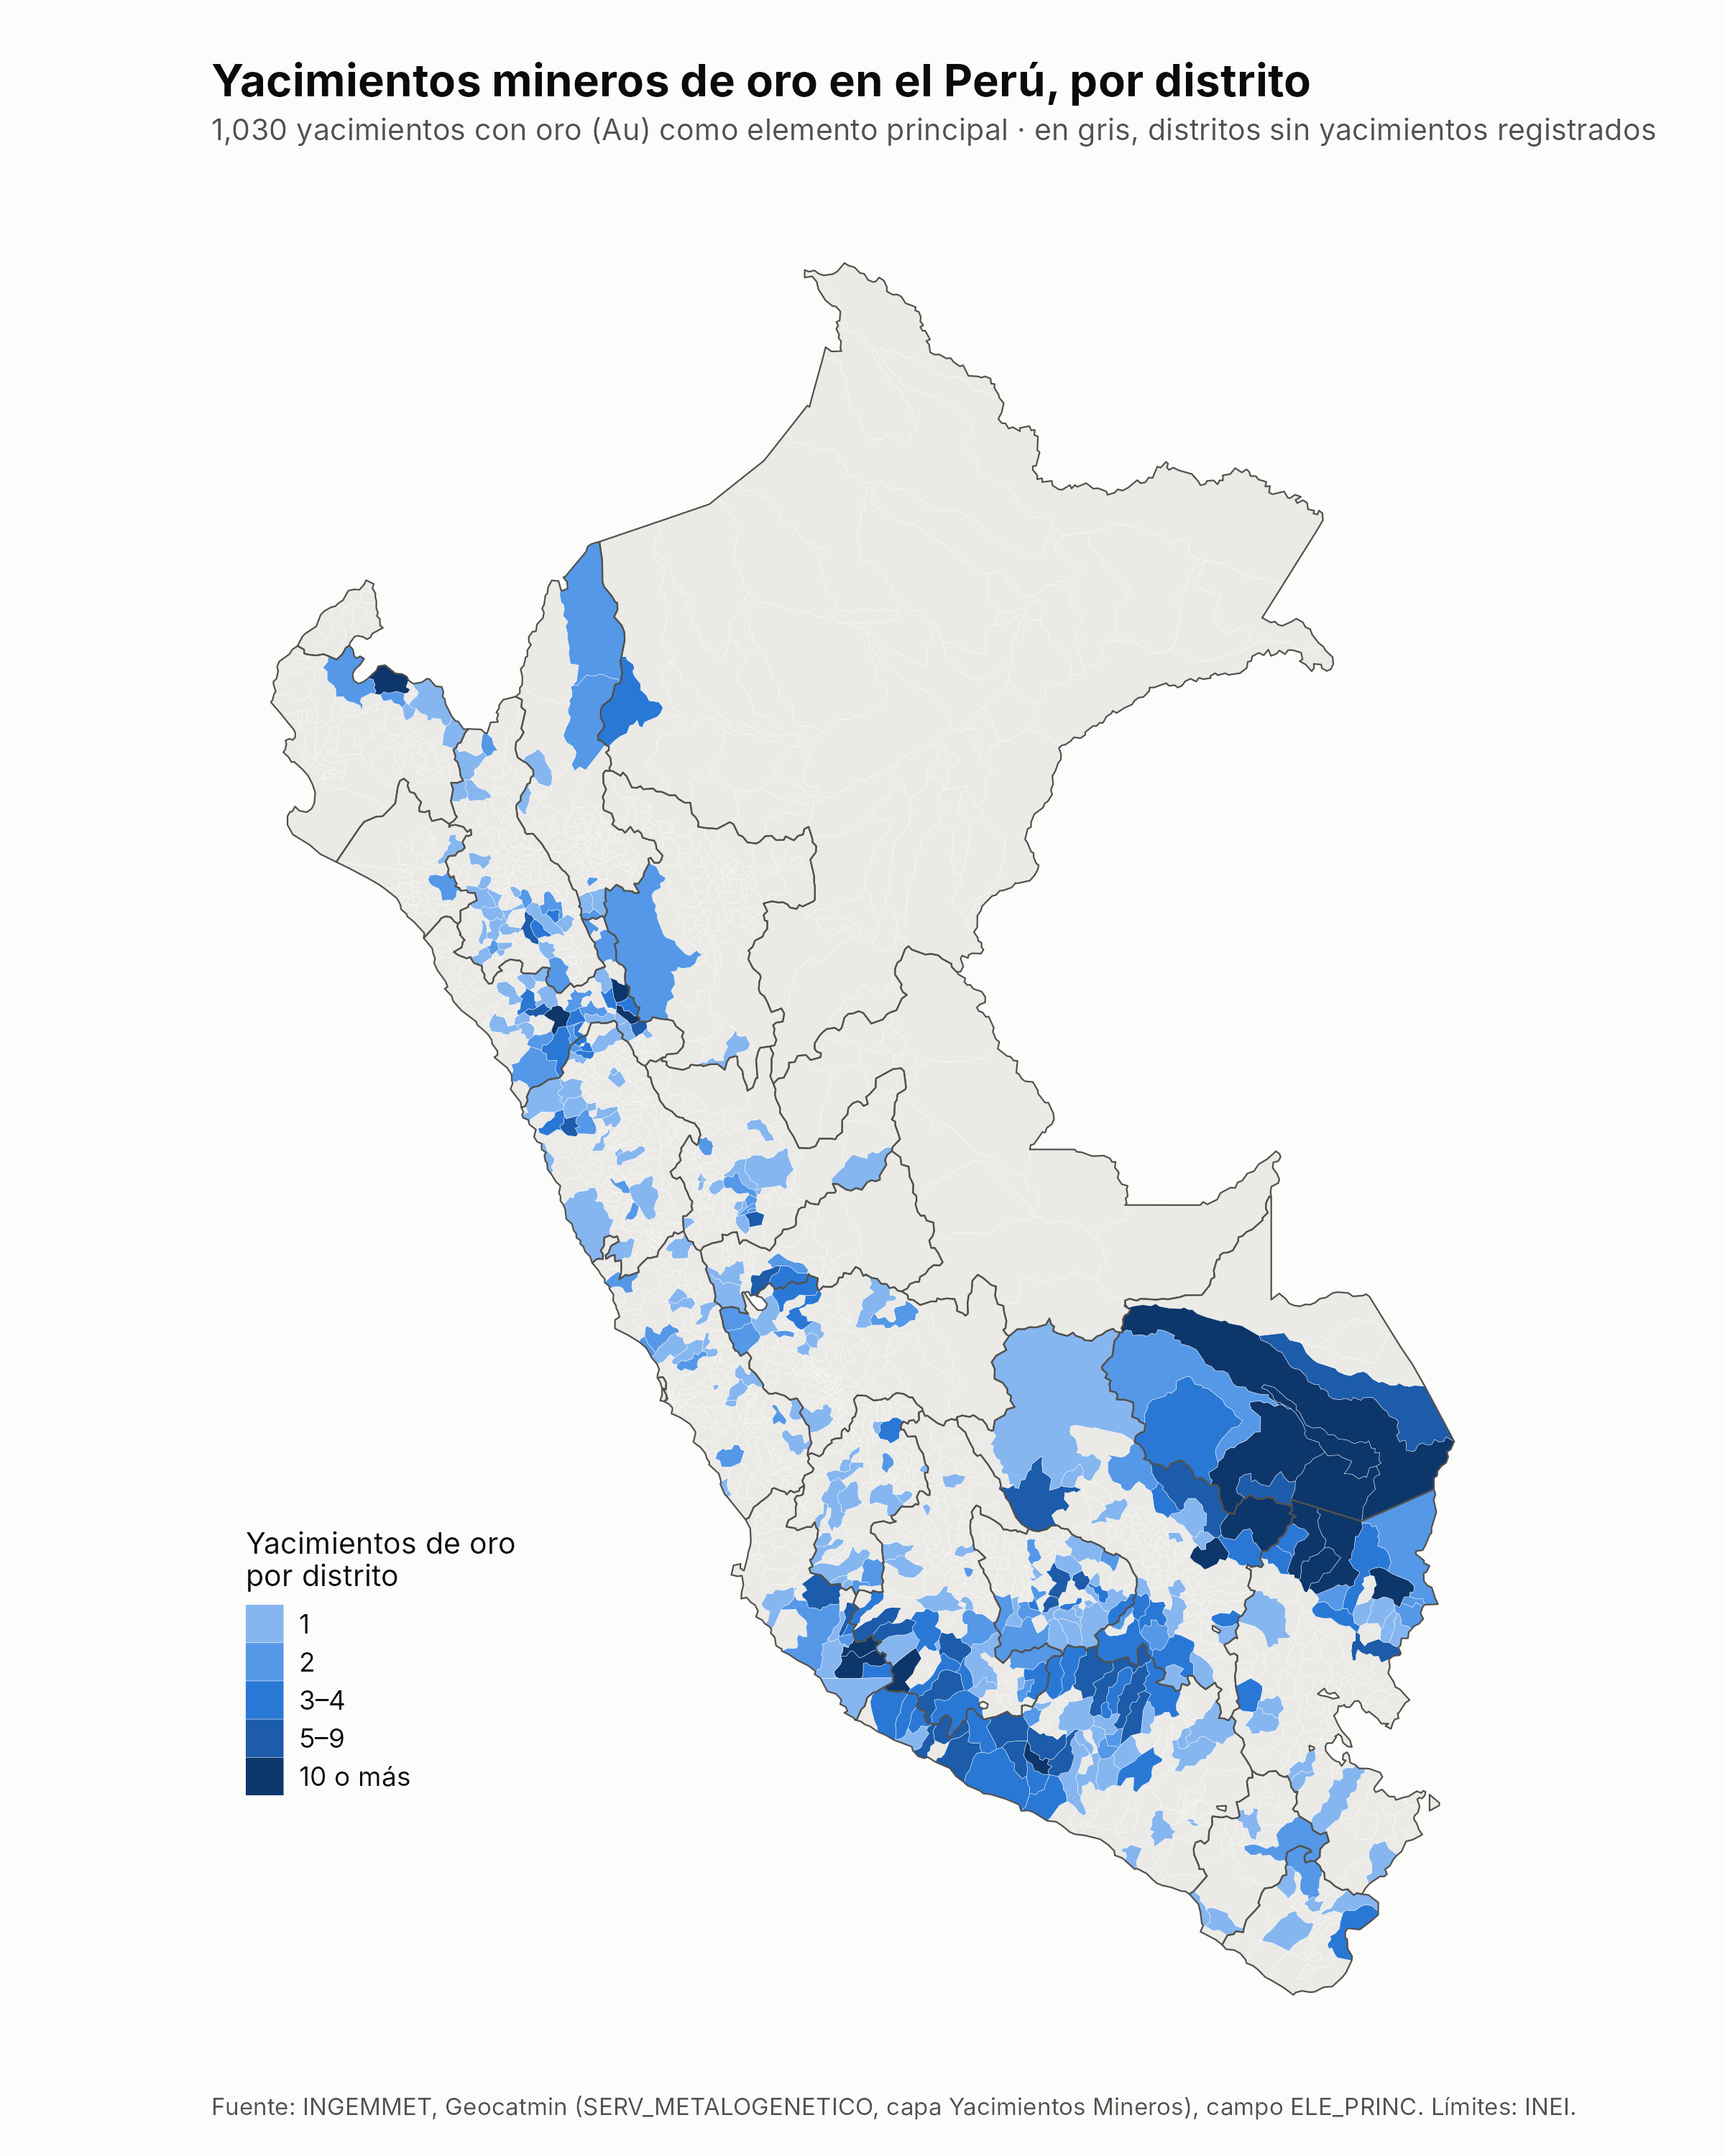
\includegraphics[width=0.85\textwidth]{mapa_oro_distritos.png}

\vspace{0.5em}
\begin{minipage}{\textwidth}
\small
\textit{Nota.} Yacimientos cuyo primer elemento principal es el oro (Au),
agrupados en cinco clases. Los distritos en gris no registran yacimientos de
oro. Las líneas oscuras corresponden a los límites departamentales.
Elaboración propia a partir de datos de GEOCATMIN \parencite{ingemmet2026} y de
límites distritales del INEI \parencite{juaneladio-geojson}.
\end{minipage}
\end{figure}

\section{Discusión}

El procedimiento permitió obtener el inventario completo de la capa de
yacimientos de GEOCATMIN y verificar en cada etapa que los conteos coincidieran
con los informados por el propio servidor. Los resultados muestran que los
yacimientos de oro registrados no se distribuyen de manera uniforme, sino que se
concentran en pocas provincias y distritos. Entre ellas destaca Tambopata, que
por sí sola reúne más del 11\,\% del total nacional.

Al interpretar estos resultados deben tenerse en cuenta varias limitaciones:

\begin{enumerate}
  \item \textit{Número de registros frente a importancia económica.} Las tablas
  y el mapa cuentan registros de yacimientos, no su tamaño, producción ni
  reservas. Además, solo el 30.6\,\% de los registros de oro son minas; el resto
  son ocurrencias (35.0\,\%), prospectos (20.9\,\%) y proyectos (13.4\,\%). Por
  ejemplo, los 145 registros de Madre de Dios corresponden en su totalidad a
  depósitos exóticos (placeres y aluviales), y la mitad de ellos (74) son
  ocurrencias. Un distrito con muchas ocurrencias o yacimientos pequeños puede
  aparecer más destacado que otro con un único yacimiento de gran escala.
  \item \textit{Efecto del tamaño de los distritos.} En un mapa coroplético, los
  distritos extensos, como los de Madre de Dios, tienen mayor peso visual que los
  distritos andinos pequeños con un número similar de yacimientos. Una
  representación alternativa sería la densidad de yacimientos por unidad de
  superficie.
  \item \textit{Criterio de selección.} Se consideró que el orden del campo
  \texttt{ELE\_PRINC} refleja la importancia relativa de los elementos. Si se
  adopta el criterio más amplio (oro en cualquier posición), el número de
  yacimientos asciende a 1184, y el archivo correspondiente también fue
  generado.
  \item \textit{Desfase de los límites distritales.} La capa de límites tiene
  1834 distritos, mientras que la división política vigente tiene 1895. Tres
  yacimientos de distritos creados recientemente se representaron en el
  distrito del que se separaron.
  \item \textit{Coherencia entre códigos y coordenadas.} Al cruzar las
  coordenadas de los yacimientos con los polígonos distritales, 54 de ellos
  (5.2\,\%) caen en un distrito distinto al indicado por su código; en 19 casos
  difiere también la provincia y en 8 el departamento. Esto puede deberse a la
  simplificación de los límites, a la precisión de las coordenadas o a cambios
  en la demarcación. Las tablas y el mapa usan el código registrado por
  INGEMMET, que es la asignación oficial de la fuente.
  \item \textit{Vigencia de los datos.} GEOCATMIN se actualiza de forma
  continua, por lo que los resultados corresponden a la fecha de consulta (12
  de octubre de 2026).
\end{enumerate}

\section{Conclusiones}

Se desarrolló un flujo de trabajo reproducible, en Python y R, para descargar los
yacimientos mineros del Perú desde GEOCATMIN, seleccionar aquellos cuyo
elemento principal es el oro y analizar su distribución territorial. El flujo
corrige dos problemas prácticos del acceso al servicio: la ubicación desactualizada
de la capa y la cadena de certificados incompleta del servidor. Esta última se
resolvió sin comprometer la seguridad de la conexión. Se identificaron 1030
yacimientos de oro, concentrados en Arequipa, Madre de Dios, La Libertad y Puno.
Las tablas por departamento, provincia y distrito y el mapa distrital pueden
regenerarse con los scripts incluidos en el repositorio para actualizar el
análisis cuando INGEMMET actualice su información.

\printbibliography

\appendix

\section{Comandos para reproducir el análisis}

Desde la raíz del repositorio, la descarga y el filtrado se ejecutan con el
script de Python:

\begin{lstlisting}
pip install requests pandas geopandas
cd datos
python ../descargar_geocatmin.py --capa 1 --salida yacimientos --oro
cd ..
\end{lstlisting}

Este comando genera los archivos \texttt{yacimientos}, \texttt{yacimientos\_oro}
y \texttt{yacimientos\_oro\_principal}, cada uno en formato CSV y GeoPackage.
Las tablas y el mapa se generan con el script de R:

\begin{lstlisting}
install.packages(c("sf", "dplyr", "readr", "ggplot2"))   # en R, una sola vez
Rscript mapa_oro_distritos.R
\end{lstlisting}

Este script produce \texttt{oro\_por\_departamento.csv},
\texttt{oro\_por\_provincia.csv}, \texttt{oro\_por\_distrito.csv} y
\texttt{mapa\_oro\_distritos.png} en la carpeta \texttt{datos/}.

\end{document}
